% Options for packages loaded elsewhere
\PassOptionsToPackage{unicode}{hyperref}
\PassOptionsToPackage{hyphens}{url}
\PassOptionsToPackage{dvipsnames,svgnames,x11names}{xcolor}
\documentclass[
  10pt,
  fontset=fandol]{ctexart}
\usepackage{xcolor}
\usepackage[margin=16mm]{geometry}
\usepackage{amsmath,amssymb}
\setcounter{secnumdepth}{-\maxdimen} % remove section numbering
\usepackage{iftex}
\ifPDFTeX
  \usepackage[T1]{fontenc}
  \usepackage[utf8]{inputenc}
  \usepackage{textcomp} % provide euro and other symbols
\else % if luatex or xetex
  \usepackage{unicode-math} % this also loads fontspec
  \defaultfontfeatures{Scale=MatchLowercase}
  \defaultfontfeatures[\rmfamily]{Ligatures=TeX,Scale=1}
\fi
\usepackage{lmodern}
\ifPDFTeX\else
  % xetex/luatex font selection
\fi
% Use upquote if available, for straight quotes in verbatim environments
\IfFileExists{upquote.sty}{\usepackage{upquote}}{}
\IfFileExists{microtype.sty}{% use microtype if available
  \usepackage[]{microtype}
  \UseMicrotypeSet[protrusion]{basicmath} % disable protrusion for tt fonts
}{}
\makeatletter
\@ifundefined{KOMAClassName}{% if non-KOMA class
  \IfFileExists{parskip.sty}{%
    \usepackage{parskip}
  }{% else
    \setlength{\parindent}{0pt}
    \setlength{\parskip}{6pt plus 2pt minus 1pt}}
}{% if KOMA class
  \KOMAoptions{parskip=half}}
\makeatother
\usepackage{longtable,booktabs,array}
\newcounter{none} % for unnumbered tables
\usepackage{calc} % for calculating minipage widths
% Correct order of tables after \paragraph or \subparagraph
\usepackage{etoolbox}
\makeatletter
\patchcmd\longtable{\par}{\if@noskipsec\mbox{}\fi\par}{}{}
\makeatother
% Allow footnotes in longtable head/foot
\IfFileExists{footnotehyper.sty}{\usepackage{footnotehyper}}{\usepackage{footnote}}
\makesavenoteenv{longtable}
\usepackage{graphicx}
\makeatletter
\newsavebox\pandoc@box
\newcommand*\pandocbounded[1]{% scales image to fit in text height/width
  \sbox\pandoc@box{#1}%
  \Gscale@div\@tempa{\textheight}{\dimexpr\ht\pandoc@box+\dp\pandoc@box\relax}%
  \Gscale@div\@tempb{\linewidth}{\wd\pandoc@box}%
  \ifdim\@tempb\p@<\@tempa\p@\let\@tempa\@tempb\fi% select the smaller of both
  \ifdim\@tempa\p@<\p@\scalebox{\@tempa}{\usebox\pandoc@box}%
  \else\usebox{\pandoc@box}%
  \fi%
}
% Set default figure placement to htbp
\def\fps@figure{htbp}
\makeatother
\setlength{\emergencystretch}{3em} % prevent overfull lines
\providecommand{\tightlist}{%
  \setlength{\itemsep}{0pt}\setlength{\parskip}{0pt}}
\usepackage{amsmath,amssymb,mathtools,needspace}
\xeCJKDeclareCharClass{CJK}{"2032,"0400->"04FF,"2160->"216B,"2460->"2473,"25A0,"25C7,"25CB,"25CF}
\IfFontExistsTF{Arial Unicode MS}{\xeCJKsetup{AutoFallBack=true}\setCJKfallbackfamilyfont{\CJKrmdefault}{Arial Unicode MS}}{}
\setcounter{secnumdepth}{0}
\setlength{\emergencystretch}{2em}
\allowdisplaybreaks
\usepackage{bookmark}
\IfFileExists{xurl.sty}{\usepackage{xurl}}{} % add URL line breaks if available
\urlstyle{same}
\hypersetup{
  pdftitle={一阶线性递推},
  colorlinks=true,
  linkcolor={Maroon},
  filecolor={Maroon},
  citecolor={Blue},
  urlcolor={Blue},
  pdfcreator={LaTeX via pandoc}}

\title{一阶线性递推}
\author{}
\date{}

\begin{document}
\maketitle

\subsection{11.3　一阶线性递推}\label{ux4e00ux9636ux7ebfux6027ux9012ux63a8}

设计串行算法的一项基本技术是递推化。递推计算采取逐步推进的方式，其每一步计算都要用到前面几步的信息。正是由于这种时序性，递推计算的并行化似乎存在实质性的困难。

设计递推计算问题的并行算法，有些学者采用了倍增技术，这种设计技术从展开式入手展示了递推问题内在的并行性。

与倍增技术不同，本节所推荐的二分技术将直接开发递推算式本身的并行性，因而设计思想更简明，使用方法更简便。这种算法设计技术可广泛应用于众多类型的递推问题。

本小节着重研究一阶线性递推问题，即寻求数列 \(x_i\)，\(i=0,1,\cdots,N-1\)，使之满足

\[
\begin{cases}
x_0=b_0,\\
x_i=a_i x_{i-1}+b_i,\quad i=1,2,\cdots,N-1,
\end{cases}
\tag{11.3.1}
\]

式中，系数 \(a_i,b_i\) 为已给。

值得指出的是，只要引进矩阵和向量的记号，总可以将高阶线性递推归结为上述一阶线性递推的情形。

\subsubsection{11.3.1　相关链的二分手续}\label{ux76f8ux5173ux94feux7684ux4e8cux5206ux624bux7eed}

为了便于刻画二分法的设计思想，首先引进相关链的概念。由于递推关系式反映了变元之间的相关性和时序性，一组有序的相关变元可抽象地表述为如下形式的相关链：

\[
\cdots\to x_{i-j}\to x_i\to\cdots,
\]

其中相邻两元素 \(x_i\) 与 \(x_{i-j}\) 的下标之差 \(j\) 称作间距。如果相关链各节的间距为定值，则将其称作步长。

对应于递推问题（11.3.1）的相关链有 \(N\) 节，即

\[
x_0\to x_1\to\cdots\to x_{N-1},
\]

\href{../../source-images/pdf-286.jpeg}{原页图像}

这里步长等于 1。

设将上述相关链按其下标的奇偶拆成两条，则每条子链含 \(N_1=N/2\) 节，即

\[
\begin{cases}
x_0\to x_2\to\cdots\to x_{N-2},\\
x_1\to x_3\to\cdots\to x_{N-1}.
\end{cases}
\tag{11.3.2}
\]

这样加工得出的递推问题有两个结果 \(x_0,x_1\)，且其步长等于 2。这是一种二分手续。

在保持结果数逐步倍增及步长逐步倍增两项基本特征的前提下反复施行这一手续，则二分 \(k\) 次后得出 \(2^k\) 个结果 \(x_i\)，\(i=0,1,\cdots,2^k-1\)，且步长增至 \(2^k\)，相应地，所给相关链被加工成 \(2^k\) 条子链，每条子链含 \(N_k=N/2^k\) 节，即

\[
\left\{
\begin{aligned}
&x_0\to x_{2^k}\to\cdots\to x_{N-2^k},\\
&x_1\to x_{2^k+1}\to\cdots\to x_{N-2^k+1},\\
&\qquad\vdots\\
&x_{2^k-1}\to x_{2^{k+1}-1}\to\cdots\to x_{N-1}.
\end{aligned}
\right.
\tag{11.3.3}
\]

如此二分 \(n=\log_2 N\) 次后，所给相关链最终退化为每条仅含一节的最简形式

\[
x_0,x_1,\cdots,x_{N-1},
\]

从而得出所求的解。

这种以下标的奇偶分离为特征的二分手续称作奇偶二分。这是最基本的一种二分手续。

对于 \(N=8\) 的具体情形，相关链的奇偶二分过程如图 11.4 所示，图中用波纹线标出每一步的新结果。

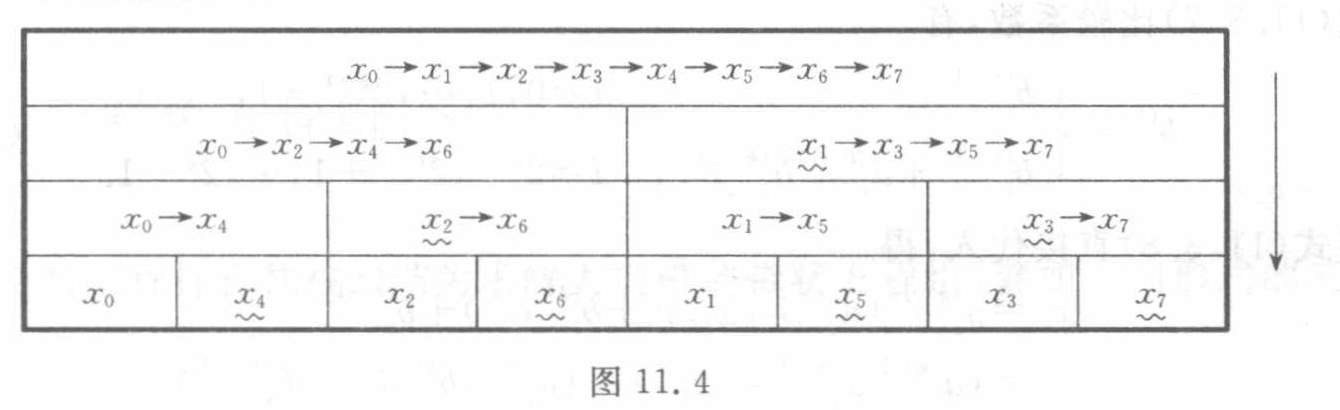
\includegraphics[width=0.85\linewidth,height=\textheight,keepaspectratio,alt={图 11.4（原图裁切）}]{../assets/ch11/figure-11-4.png}

图 11.4　原图右侧箭头向下，逐层由左至右的全部相关链与波纹线标记如下：

{\def\LTcaptype{none} % do not increment counter
\begin{longtable}[]{@{}
  >{\raggedright\arraybackslash}p{(\linewidth - 4\tabcolsep) * \real{0.3333}}
  >{\raggedright\arraybackslash}p{(\linewidth - 4\tabcolsep) * \real{0.3333}}
  >{\raggedright\arraybackslash}p{(\linewidth - 4\tabcolsep) * \real{0.3333}}@{}}
\toprule\noalign{}
\begin{minipage}[b]{\linewidth}\raggedright
层次（由上至下）
\end{minipage} & \begin{minipage}[b]{\linewidth}\raggedright
相关链或单节
\end{minipage} & \begin{minipage}[b]{\linewidth}\raggedright
波纹线标出的新结果
\end{minipage} \\
\midrule\noalign{}
\endhead
\bottomrule\noalign{}
\endlastfoot
初始层 & \(x_0\to x_1\to x_2\to x_3\to x_4\to x_5\to x_6\to x_7\) & 无 \\
第 1 次二分 & \(x_0\to x_2\to x_4\to x_6\)；\(x_1\to x_3\to x_5\to x_7\) & \(x_1\) \\
第 2 次二分 & \(x_0\to x_4\)；\(x_2\to x_6\)；\(x_1\to x_5\)；\(x_3\to x_7\) & \(x_2,x_3\) \\
第 3 次二分 & \(x_0\)；\(x_4\)；\(x_2\)；\(x_6\)；\(x_1\)；\(x_5\)；\(x_3\)；\(x_7\) & \(x_4,x_6,x_5,x_7\) \\
\end{longtable}
}

（上表为原图标签与结构的文字转录。）

\subsubsection{11.3.2　算式的建立}\label{ux7b97ux5f0fux7684ux5efaux7acb}

现在运用消元手续具体建立上述奇偶二分法的算式。回到递推问题（11.3.1），利用它的第 \(i-1\) 式从其第 \(i\) 式中消去 \(x_{i-1}\)，得

\[
\begin{cases}
x_i=b_i^{(1)},& i=0,1,\\
x_i=a_i^{(1)}x_{i-2}+b_i^{(1)},& i=2,3,\cdots,N-1,
\end{cases}
\tag{11.3.4}
\]

式中

\[
a_i^{(1)}=a_i a_{i-1},\quad i=2,3,\cdots,N-1,
\tag{11.3.5}
\]

\href{../../source-images/pdf-287.jpeg}{原页图像}

\[
b_i^{(1)}=
\begin{cases}
b_i,& i=0,\\
b_i+a_i b_{i-1},& i=1,2,\cdots,N-1.
\end{cases}
\tag{11.3.6}
\]

容易看出，式（11.3.4）可按下标的奇偶拆成两个规模减半的子问题，即

\[
\begin{cases}
x_0=b_0^{(1)},\\
x_{2i}=a_{2i}^{(1)}x_{2i-2}+b_{2i}^{(1)},\quad i=1,2,\cdots,N_1-1;
\end{cases}
\]

\[
\begin{cases}
x_1=b_1^{(1)},\\
x_{2i+1}=a_{2i+1}^{(1)}x_{2i-1}+b_{2i+1}^{(1)},\quad i=1,2,\cdots,N_1-1.
\end{cases}
\]

它们分别对应于形如式（11.3.2）的奇偶相关链。

前已指出，二分 \(k\) 步后加工得出的相关链式（11.3.3）含有 \(2^k\) 个结果 \(x_i\)，\(i=0,1,\cdots,2^k-1\)，且其步长增至 \(2^k\)，因此其相应的递推问题具有如下形式：

\[
\begin{cases}
x_i=b_i^{(k)},& i=0,1,\cdots,2^k-1,\\
x_i=a_i^{(k)}x_{i-2^k}+b_i^{(k)},& i=2^k,2^k+1,\cdots,N-1.
\end{cases}
\tag{11.3.7}
\]

为了导出系数 \(a_i^{(k)},b_i^{(k)}\) 的计算公式，回到前一步加工得出的递推问题：

\[
\begin{cases}
x_i=b_i^{(k-1)},& i=0,1,\cdots,2^{k-1}-1,\\
x_i=a_i^{(k-1)}x_{i-2^{k-1}}+b_i^{(k-1)},& i=2^{k-1},2^{k-1}+1,\cdots,N-1.
\end{cases}
\tag{11.3.8}
\]

显然，据此可得出 \(2^{k-1}\) 个新结果

\[
x_i=a_i^{(k-1)}b_{i-2^{k-1}}^{(k-1)}+b_i^{(k-1)},\quad i=2^{k-1},2^{k-1}+1,\cdots,2^k-1,
\]

与式（11.3.7）比较系数，有

\[
b_i^{(k)}=
\begin{cases}
b_i^{(k-1)},& i=0,1,\cdots,2^{k-1}-1,\\
b_i^{(k-1)}+a_i^{(k-1)}b_{i-2^{k-1}}^{(k-1)},& i=2^{k-1},2^{k-1}+1,\cdots,2^k-1.
\end{cases}
\tag{11.3.9}
\]

又将式（11.3.8）直接代入，得

\[
\begin{aligned}
x_i
&=a_i^{(k-1)}\left(a_{i-2^{k-1}}^{(k-1)}x_{i-2^k}+b_{i-2^{k-1}}^{(k-1)}\right)+b_i^{(k-1)}\\
&=\left(a_i^{(k-1)}a_{i-2^{k-1}}^{(k-1)}\right)x_{i-2^k}+\left(a_i^{(k-1)}b_{i-2^{k-1}}^{(k-1)}+b_i^{(k-1)}\right).
\end{aligned}
\]

再与式（11.3.7）比较系数，知

\[
\left\{
\begin{aligned}
a_i^{(k)}&=a_i^{(k-1)}a_{i-2^{k-1}}^{(k-1)},\\
b_i^{(k)}&=b_i^{(k-1)}+a_i^{(k-1)}b_{i-2^{k-1}}^{(k-1)},
\end{aligned}
\right.
\quad i=2^k,2^k+1,\cdots,N-1.
\]

将计算 \(b_i^{(k)}\) 的上述两组算式归并在一起，即可归纳出求解递推问题的奇偶二分算法 11.4。

\textbf{算法 11.4}　对 \(k=1,2,\cdots\) 直到 \(n=\log_2 N\) 执行算式

\[
a_i^{(k)}=a_i^{(k-1)}a_{i-2^{k-1}}^{(k-1)},\quad i=2^k,2^{k+1},\cdots,N-1;
\tag{11.3.10}
\]

\[
b_i^{(k)}=
\begin{cases}
b_i^{(k-1)},& i=0,1,\cdots,2^{k-1}-1,\\
b_i^{(k-1)}+a_i^{(k-1)}b_{i-2^{k-1}}^{(k-1)},& i=2^{k-1},2^{k-1}+1,\cdots,N-1,
\end{cases}
\tag{11.3.11}
\]

\begin{quote}
校注（agent 补充，CH11-E003）：式（11.3.10）中的下标序列确实印为 \(i=2^k,2^{k+1},\cdots,N-1\)，已按放大原图照录。与本页上方推导及式（11.3.7）的逐个下标范围比较，此处第二项疑应为 \(2^k+1\)，而不是 \(2^{k+1}\)；属于原书排印疑误。
\end{quote}

\href{../../source-images/pdf-288.jpeg}{原页图像}

则 \(x_i=b_i^{(n)}\)，\(i=0,1,\cdots,N-1\) 即为所求。

\subsubsection{11.3.3　二分算法的效能分析}\label{ux4e8cux5206ux7b97ux6cd5ux7684ux6548ux80fdux5206ux6790}

考察奇偶二分法的算法 11.4。按式（11.3.10）、式（11.3.11），每一步需做两次运算（乘法、加法各一次），共做 \(n=\log_2 N\) 步，故其时间界为

\[
T^*=2\log_2 N.
\]

再考察该算法的第 \(k\) 步。为使每个系数 \(a_i^{(k)},b_i^{(k)}\) 各有一台处理机去独立计算，则按式（11.3.10）、式（11.3.11）计算所需的处理机台数为

\[
P_k=(N-2^k)+(N-2^{k-1})=2N-3\times2^{k-1}.
\]

因此，该算法的处理机台数界为

\[
P^*=\max_{1\le k\le n}P_k\approx2N.
\]

注意到一阶线性递推问题串行计算的运行时间 \(T_1=2(N-1)\)，可知奇偶二分法的加速比

\[
S=\frac{T_1}{T^*}\approx\frac{N}{\log_2 N},
\]

而其效率

\[
E=\frac{S}{P^*}\approx\frac{1}{2\log_2 N}.
\]

这一算法同叠加计算的二分法（11.2.5 小节）具有相同的加速比，只是效率降低了。

\subsection{本节覆盖原页的校注记录}\label{ux672cux8282ux8986ux76d6ux539fux9875ux7684ux6821ux6ce8ux8bb0ux5f55}

下列记录按原页关联，含同页相邻小节的校注；计算时同时读取上文校注和完整原页。

\begin{itemize}
\tightlist
\item
  \texttt{CH11-E003}：原书 PDF 页 287
\end{itemize}

\end{document}
